\documentclass[12pt,landscape]{article}

%\usepackage{lmodern}
\usepackage{amssymb,amsmath}
\usepackage{bm}
\usepackage{graphicx}
\usepackage{microtype}
\usepackage{hyperref}
\pagestyle{empty}
\usepackage{titlesec}
\titleformat*{\section}{\LARGE\bfseries}
\titleformat*{\subsection}{\LARGE\bfseries}
\titleformat*{\subsubsection}{\LARGE\bfseries}
\setlength{\parindent}{0pt}
\setlength{\parskip}{1.2ex}
\setlength{\parindent}{0pt}
\setlength{\parskip}{1.2ex}

\setlength{\oddsidemargin}{-16mm}
\setlength{\textwidth}{260mm}
\setlength{\columnsep}{0.5in}
\setlength{\columnseprule}{1pt}
\setlength{\textheight}{202mm}
\setlength{\topmargin}{-32mm}
\setlength{\headsep}{0.25in}

\hypersetup
       {   pdfauthor = { Marco Fasondini },
           pdftitle={ foo },
           colorlinks=TRUE,
           linkcolor=black,
           citecolor=blue,
           urlcolor=blue
       }




\usepackage{upquote}
\usepackage{listings}
\usepackage{xcolor}
\lstset{
    basicstyle=\ttfamily\footnotesize,
    upquote=true,
    breaklines=true,
    breakindent=0pt,
    keepspaces=true,
    showspaces=false,
    columns=fullflexible,
    showtabs=false,
    showstringspaces=false,
    escapeinside={(*@}{@*)},
    extendedchars=true,
}
\newcommand{\HLJLt}[1]{#1}
\newcommand{\HLJLw}[1]{#1}
\newcommand{\HLJLe}[1]{#1}
\newcommand{\HLJLeB}[1]{#1}
\newcommand{\HLJLo}[1]{#1}
\newcommand{\HLJLk}[1]{\textcolor[RGB]{148,91,176}{\textbf{#1}}}
\newcommand{\HLJLkc}[1]{\textcolor[RGB]{59,151,46}{\textit{#1}}}
\newcommand{\HLJLkd}[1]{\textcolor[RGB]{214,102,97}{\textit{#1}}}
\newcommand{\HLJLkn}[1]{\textcolor[RGB]{148,91,176}{\textbf{#1}}}
\newcommand{\HLJLkp}[1]{\textcolor[RGB]{148,91,176}{\textbf{#1}}}
\newcommand{\HLJLkr}[1]{\textcolor[RGB]{148,91,176}{\textbf{#1}}}
\newcommand{\HLJLkt}[1]{\textcolor[RGB]{148,91,176}{\textbf{#1}}}
\newcommand{\HLJLn}[1]{#1}
\newcommand{\HLJLna}[1]{#1}
\newcommand{\HLJLnb}[1]{#1}
\newcommand{\HLJLnbp}[1]{#1}
\newcommand{\HLJLnc}[1]{#1}
\newcommand{\HLJLncB}[1]{#1}
\newcommand{\HLJLnd}[1]{\textcolor[RGB]{214,102,97}{#1}}
\newcommand{\HLJLne}[1]{#1}
\newcommand{\HLJLneB}[1]{#1}
\newcommand{\HLJLnf}[1]{\textcolor[RGB]{66,102,213}{#1}}
\newcommand{\HLJLnfm}[1]{\textcolor[RGB]{66,102,213}{#1}}
\newcommand{\HLJLnp}[1]{#1}
\newcommand{\HLJLnl}[1]{#1}
\newcommand{\HLJLnn}[1]{#1}
\newcommand{\HLJLno}[1]{#1}
\newcommand{\HLJLnt}[1]{#1}
\newcommand{\HLJLnv}[1]{#1}
\newcommand{\HLJLnvc}[1]{#1}
\newcommand{\HLJLnvg}[1]{#1}
\newcommand{\HLJLnvi}[1]{#1}
\newcommand{\HLJLnvm}[1]{#1}
\newcommand{\HLJLl}[1]{#1}
\newcommand{\HLJLld}[1]{\textcolor[RGB]{148,91,176}{\textit{#1}}}
\newcommand{\HLJLs}[1]{\textcolor[RGB]{201,61,57}{#1}}
\newcommand{\HLJLsa}[1]{\textcolor[RGB]{201,61,57}{#1}}
\newcommand{\HLJLsb}[1]{\textcolor[RGB]{201,61,57}{#1}}
\newcommand{\HLJLsc}[1]{\textcolor[RGB]{201,61,57}{#1}}
\newcommand{\HLJLsd}[1]{\textcolor[RGB]{201,61,57}{#1}}
\newcommand{\HLJLsdB}[1]{\textcolor[RGB]{201,61,57}{#1}}
\newcommand{\HLJLsdC}[1]{\textcolor[RGB]{201,61,57}{#1}}
\newcommand{\HLJLse}[1]{\textcolor[RGB]{59,151,46}{#1}}
\newcommand{\HLJLsh}[1]{\textcolor[RGB]{201,61,57}{#1}}
\newcommand{\HLJLsi}[1]{#1}
\newcommand{\HLJLso}[1]{\textcolor[RGB]{201,61,57}{#1}}
\newcommand{\HLJLsr}[1]{\textcolor[RGB]{201,61,57}{#1}}
\newcommand{\HLJLss}[1]{\textcolor[RGB]{201,61,57}{#1}}
\newcommand{\HLJLssB}[1]{\textcolor[RGB]{201,61,57}{#1}}
\newcommand{\HLJLnB}[1]{\textcolor[RGB]{59,151,46}{#1}}
\newcommand{\HLJLnbB}[1]{\textcolor[RGB]{59,151,46}{#1}}
\newcommand{\HLJLnfB}[1]{\textcolor[RGB]{59,151,46}{#1}}
\newcommand{\HLJLnh}[1]{\textcolor[RGB]{59,151,46}{#1}}
\newcommand{\HLJLni}[1]{\textcolor[RGB]{59,151,46}{#1}}
\newcommand{\HLJLnil}[1]{\textcolor[RGB]{59,151,46}{#1}}
\newcommand{\HLJLnoB}[1]{\textcolor[RGB]{59,151,46}{#1}}
\newcommand{\HLJLoB}[1]{\textcolor[RGB]{102,102,102}{\textbf{#1}}}
\newcommand{\HLJLow}[1]{\textcolor[RGB]{102,102,102}{\textbf{#1}}}
\newcommand{\HLJLp}[1]{#1}
\newcommand{\HLJLc}[1]{\textcolor[RGB]{153,153,119}{\textit{#1}}}
\newcommand{\HLJLch}[1]{\textcolor[RGB]{153,153,119}{\textit{#1}}}
\newcommand{\HLJLcm}[1]{\textcolor[RGB]{153,153,119}{\textit{#1}}}
\newcommand{\HLJLcp}[1]{\textcolor[RGB]{153,153,119}{\textit{#1}}}
\newcommand{\HLJLcpB}[1]{\textcolor[RGB]{153,153,119}{\textit{#1}}}
\newcommand{\HLJLcs}[1]{\textcolor[RGB]{153,153,119}{\textit{#1}}}
\newcommand{\HLJLcsB}[1]{\textcolor[RGB]{153,153,119}{\textit{#1}}}
\newcommand{\HLJLg}[1]{#1}
\newcommand{\HLJLgd}[1]{#1}
\newcommand{\HLJLge}[1]{#1}
\newcommand{\HLJLgeB}[1]{#1}
\newcommand{\HLJLgh}[1]{#1}
\newcommand{\HLJLgi}[1]{#1}
\newcommand{\HLJLgo}[1]{#1}
\newcommand{\HLJLgp}[1]{#1}
\newcommand{\HLJLgs}[1]{#1}
\newcommand{\HLJLgsB}[1]{#1}
\newcommand{\HLJLgt}[1]{#1}



\def\qqand{\qquad\hbox{and}\qquad}
\def\qqfor{\qquad\hbox{for}\qquad}
\def\qqas{\qquad\hbox{as}\qquad}
\def\half{ {1 \over 2} }
\def\D{ {\rm d} }
\def\I{ {\rm i} }
\def\E{ {\rm e} }
\def\C{ {\mathbb C} }
\def\R{ {\mathbb R} }
\def\H{ {\mathbb H} }
\def\Z{ {\mathbb Z} }
\def\CC{ {\cal C} }
\def\FF{ {\cal F} }
\def\HH{ {\cal H} }
\def\LL{ {\cal L} }
\def\vc#1{ {\mathbf #1} }
\def\bbC{ {\mathbb C} }



\def\fR{ f_{\rm R} }
\def\fL{ f_{\rm L} }

\def\qqqquad{\qquad\qquad}
\def\qqwhere{\qquad\hbox{where}\qquad}
\def\Res_#1{\underset{#1}{\rm Res}\,}
\def\sech{ {\rm sech}\, }
\def\acos{ {\rm acos}\, }
\def\asin{ {\rm asin}\, }
\def\atan{ {\rm atan}\, }
\def\Ei{ {\rm Ei}\, }
\def\upepsilon{\varepsilon}


\def\Xint#1{ \mathchoice
   {\XXint\displaystyle\textstyle{#1} }%
   {\XXint\textstyle\scriptstyle{#1} }%
   {\XXint\scriptstyle\scriptscriptstyle{#1} }%
   {\XXint\scriptscriptstyle\scriptscriptstyle{#1} }%
   \!\int}
\def\XXint#1#2#3{ {\setbox0=\hbox{$#1{#2#3}{\int}$}
     \vcenter{\hbox{$#2#3$}}\kern-.5\wd0} }
\def\ddashint{\Xint=}
\def\dashint{\Xint-}
% \def\dashint
\def\infdashint{\dashint_{-\infty}^\infty}




\def\addtab#1={#1\;&=}
\def\ccr{\\\addtab}
\def\ip<#1>{\left\langle{#1}\right\rangle}
\def\dx{\D x}
\def\dt{\D t}
\def\dz{\D z}
\def\ds{\D s}

\def\rR{ {\rm R} }
\def\rL{ {\rm L} }

\def\norm#1{\left\| #1 \right\|}

\def\pr(#1){\left({#1}\right)}
\def\br[#1]{\left[{#1}\right]}

\def\abs#1{\left|{#1}\right|}
\def\fpr(#1){\!\pr({#1})}

\def\sopmatrix#1{ \begin{pmatrix}#1\end{pmatrix} }

\def\endash{–}
\def\emdash{—}
\def\mdblksquare{\blacksquare}
\def\lgblksquare{\blacksquare}
\def\scre{\E}
\def\mapengine#1,#2.{\mapfunction{#1}\ifx\void#2\else\mapengine #2.\fi }

\def\map[#1]{\mapengine #1,\void.}

\def\mapenginesep_#1#2,#3.{\mapfunction{#2}\ifx\void#3\else#1\mapengine #3.\fi }

\def\mapsep_#1[#2]{\mapenginesep_{#1}#2,\void.}


\def\vcbr[#1]{\pr(#1)}


\def\bvect[#1,#2]{
{
\def\dots{\cdots}
\def\mapfunction##1{\ | \  ##1}
	\sopmatrix{
		 \,#1\map[#2]\,
	}
}
}



\def\vect[#1]{
{\def\dots{\ldots}
	\vcbr[{#1}]
} }

\def\vectt[#1]{
{\def\dots{\ldots}
	\vect[{#1}]^{\top}
} }

\def\Vectt[#1]{
{
\def\mapfunction##1{##1 \cr}
\def\dots{\vdots}
	\begin{pmatrix}
		\map[#1]
	\end{pmatrix}
} }

\def\addtab#1={#1\;&=}
\def\ccr{\\\addtab}

\def\questionequals{= \!\!\!\!\!\!{\scriptstyle ? \atop }\,\,\,}

\def\cent#1{\begin{center}#1\end{center} }

\lstset{
    basicstyle=\ttfamily,
	}

\begin{document}
{\LARGE
\sf
\textbf{Applied Complex Analysis (2021)}

\section{Lecture 10: Branch cuts}
We now discuss functions with branch cuts

\begin{itemize}
\item[1. ] Logarithm: $\log z$ with a cut on $(-\infty,0]$


\item[2. ] Powers: $z^\alpha$ with a cut on $(-\infty,0]$


\item[3. ] Combinations: $\sqrt{z-1}\sqrt{z+1}$ with a cut on $[-1,1]$

\end{itemize}
This is a step towards Cauchy transforms on cuts, for recovering a holomorphic function from its behaviour on a cut. This lecture we discuss:

\begin{itemize}
\item[1. ] Complex logarithm


\item[2. ] Algebraic powers


\item[3. ] Inferring analyticity from continuity

\end{itemize}
\newpage
\subsection{Complex logarithm}
One way to define the logarithm is as $\log|z| + \I \arg z$. We find it more convenient in order to understand its behaviour to define it as an integral:

\textbf{Definition (Complex Logarithm)}

\[
\log z := \int_1^z {1 \over \zeta} \D\zeta
\]
where the integral is understood to be on a straight line segment, that is

\[
\log z := \int_{\gamma_z} {1 \over \zeta} d\zeta
\]
where $\gamma_z(t) = 1 + (z-1)t$ for $0 \leq t \leq 1$.
\newpage
\emph{Demonstration} this shows the integral path for a point $z$. We see how the path avoids the pole of $\zeta^{-1}$ at the origin:


\begin{lstlisting}
(*@\HLJLk{using}@*) (*@\HLJLn{Plots}@*)(*@\HLJLp{,}@*) (*@\HLJLn{ComplexPhasePortrait}@*)(*@\HLJLp{,}@*) (*@\HLJLn{ApproxFun}@*)
(*@\HLJLn{z}@*) (*@\HLJLoB{=}@*) (*@\HLJLoB{-}@*)(*@\HLJLni{2}@*) (*@\HLJLoB{+}@*) (*@\HLJLnfB{1.0}@*)(*@\HLJLn{im}@*)
(*@\HLJLnf{phaseplot}@*)(*@\HLJLp{(}@*)(*@\HLJLoB{-}@*)(*@\HLJLnfB{3..3}@*)(*@\HLJLp{,}@*) (*@\HLJLoB{-}@*)(*@\HLJLnfB{3..3}@*)(*@\HLJLp{,}@*) (*@\HLJLn{\ensuremath{\zeta}}@*) (*@\HLJLoB{->}@*) (*@\HLJLni{1}@*)(*@\HLJLoB{/}@*)(*@\HLJLn{\ensuremath{\zeta}}@*)(*@\HLJLp{)}@*)
(*@\HLJLn{t}@*) (*@\HLJLoB{=}@*) (*@\HLJLni{0}@*)(*@\HLJLoB{:}@*)(*@\HLJLnfB{0.1}@*)(*@\HLJLoB{:}@*)(*@\HLJLni{1}@*)
(*@\HLJLn{\ensuremath{\gamma}}@*) (*@\HLJLoB{=}@*) (*@\HLJLni{1}@*) (*@\HLJLoB{.+}@*) (*@\HLJLp{(}@*)(*@\HLJLn{z}@*)(*@\HLJLoB{-}@*)(*@\HLJLni{1}@*)(*@\HLJLp{)}@*)(*@\HLJLoB{*}@*)(*@\HLJLn{t}@*)
(*@\HLJLnf{plot!}@*)(*@\HLJLp{(}@*)(*@\HLJLn{real}@*)(*@\HLJLoB{.}@*)(*@\HLJLp{(}@*)(*@\HLJLn{\ensuremath{\gamma}}@*)(*@\HLJLp{),}@*) (*@\HLJLn{imag}@*)(*@\HLJLoB{.}@*)(*@\HLJLp{(}@*)(*@\HLJLn{\ensuremath{\gamma}}@*)(*@\HLJLp{);}@*) (*@\HLJLn{color}@*)(*@\HLJLoB{=:}@*)(*@\HLJLn{black}@*)(*@\HLJLp{,}@*) (*@\HLJLn{label}@*)(*@\HLJLoB{=}@*)(*@\HLJLs{"{}contour"{}}@*)(*@\HLJLp{,}@*) (*@\HLJLn{arrow}@*)(*@\HLJLoB{=}@*)(*@\HLJLkc{true}@*)(*@\HLJLp{)}@*)
\end{lstlisting}

\cent{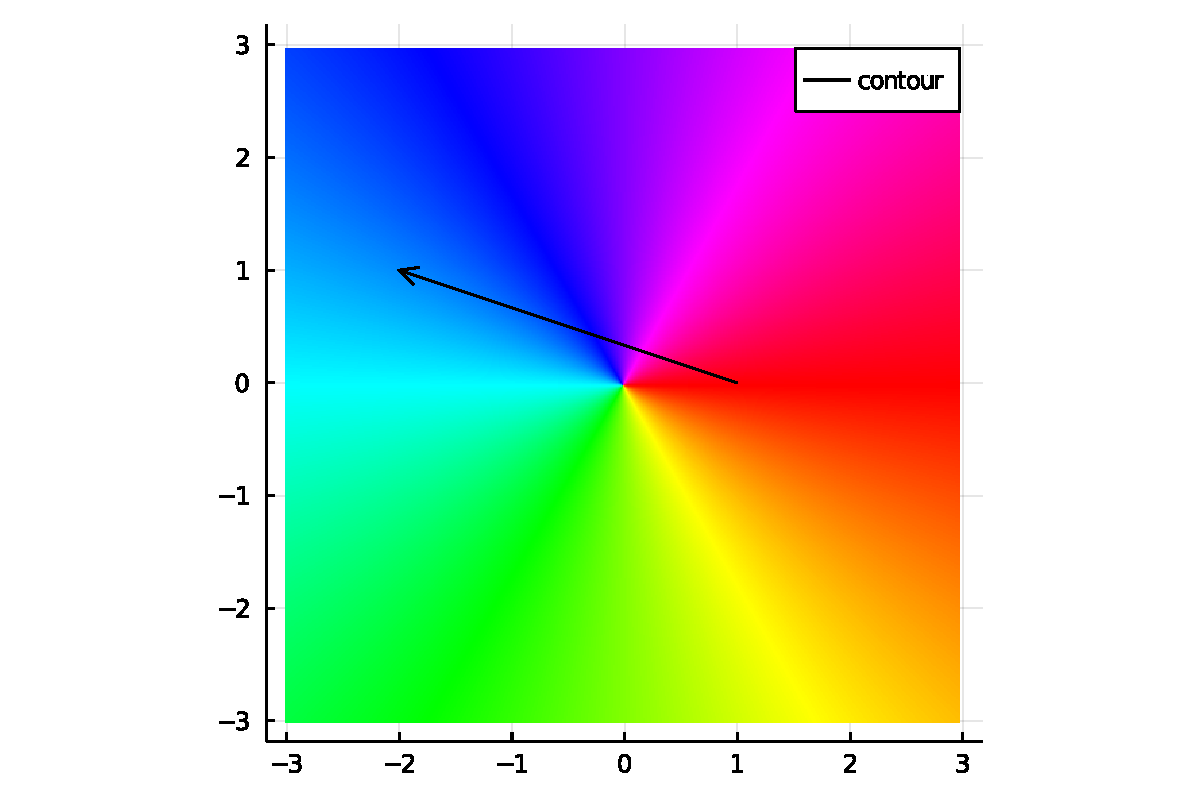
\includegraphics[width=0.5\linewidth]{C:/Users/mfaso/OneDrive/Documents/GitHub/M3M6AppliedComplexAnalysis/output/figures/Lecture10_1_1.pdf}}

This is well-defined apart from $z \in (-\infty,0]$, where there is a pole on the contour. This induces a \emph{branch cut}: a jump in the value of the function, which can be clearly seen from a phase portrait:


\begin{lstlisting}
(*@\HLJLnf{phaseplot}@*)(*@\HLJLp{(}@*)(*@\HLJLoB{-}@*)(*@\HLJLnfB{3..3}@*)(*@\HLJLp{,}@*) (*@\HLJLoB{-}@*)(*@\HLJLnfB{3..3}@*)(*@\HLJLp{,}@*) (*@\HLJLn{z}@*) (*@\HLJLoB{->}@*) (*@\HLJLnf{log}@*)(*@\HLJLp{(}@*)(*@\HLJLn{z}@*)(*@\HLJLp{))}@*)
\end{lstlisting}

\cent{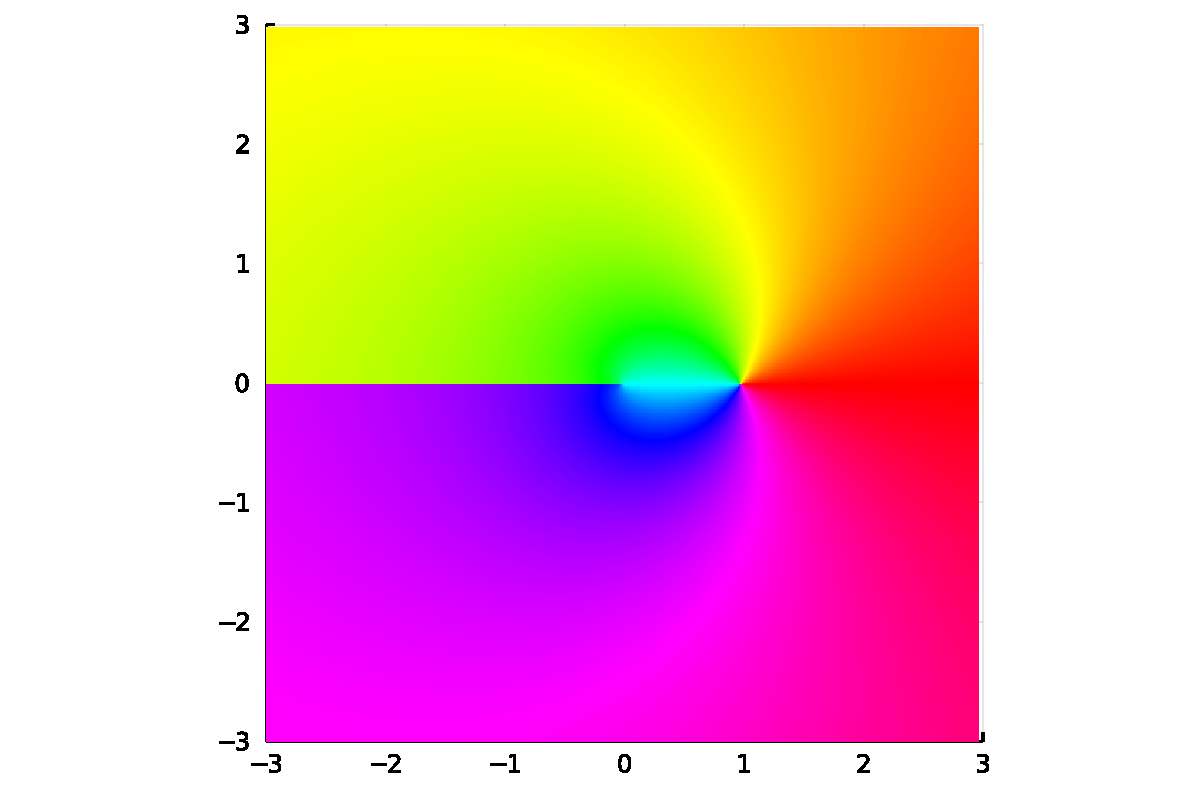
\includegraphics[width=0.8\linewidth]{C:/Users/mfaso/OneDrive/Documents/GitHub/M3M6AppliedComplexAnalysis/output/figures/Lecture10_2_1.pdf}}

We see that the limits from above and below exist: we can define
\begin{align*}
\log_+ x &:= \lim_{\epsilon \rightarrow 0^+} \log(x+\I \epsilon) \\
\log_- x &:= \lim_{\epsilon \rightarrow 0^+} \log(x-\I \epsilon)
\end{align*}
\newpage
By deformation of contours, the value of the integrals is independent of the path. Here we calculate the integral on an arc:


\begin{lstlisting}
(*@\HLJLn{\ensuremath{\theta}}@*) (*@\HLJLoB{=}@*) (*@\HLJLnf{range}@*)(*@\HLJLp{(}@*)(*@\HLJLni{0}@*)(*@\HLJLp{,}@*) (*@\HLJLn{stop}@*)(*@\HLJLoB{=}@*)(*@\HLJLnfB{0.9}@*)(*@\HLJLn{\ensuremath{\pi}}@*)(*@\HLJLp{,}@*) (*@\HLJLn{length}@*)(*@\HLJLoB{=}@*)(*@\HLJLni{100}@*)(*@\HLJLp{)}@*)
(*@\HLJLn{a}@*) (*@\HLJLoB{=}@*) (*@\HLJLn{exp}@*)(*@\HLJLoB{.}@*)(*@\HLJLp{(}@*)(*@\HLJLn{im}@*)(*@\HLJLoB{*}@*)(*@\HLJLn{\ensuremath{\theta}}@*)(*@\HLJLp{)}@*)
(*@\HLJLn{z}@*) (*@\HLJLoB{=}@*) (*@\HLJLnf{exp}@*)(*@\HLJLp{(}@*)(*@\HLJLnfB{0.9}@*)(*@\HLJLoB{*}@*)(*@\HLJLn{\ensuremath{\pi}}@*)(*@\HLJLoB{*}@*)(*@\HLJLn{im}@*)(*@\HLJLp{)}@*)
(*@\HLJLn{\ensuremath{\gamma}}@*) (*@\HLJLoB{=}@*) (*@\HLJLni{1}@*) (*@\HLJLoB{.+}@*) (*@\HLJLp{(}@*)(*@\HLJLn{z}@*)(*@\HLJLoB{-}@*)(*@\HLJLni{1}@*)(*@\HLJLp{)}@*)(*@\HLJLoB{*}@*)(*@\HLJLn{t}@*)
(*@\HLJLnf{phaseplot}@*)(*@\HLJLp{(}@*)(*@\HLJLoB{-}@*)(*@\HLJLnfB{3..3}@*)(*@\HLJLp{,}@*) (*@\HLJLoB{-}@*)(*@\HLJLnfB{3..3}@*)(*@\HLJLp{,}@*) (*@\HLJLn{\ensuremath{\zeta}}@*) (*@\HLJLoB{->}@*) (*@\HLJLni{1}@*)(*@\HLJLoB{/}@*)(*@\HLJLn{\ensuremath{\zeta}}@*)(*@\HLJLp{)}@*)
(*@\HLJLnf{plot!}@*)(*@\HLJLp{(}@*)(*@\HLJLn{real}@*)(*@\HLJLoB{.}@*)(*@\HLJLp{(}@*)(*@\HLJLn{\ensuremath{\gamma}}@*)(*@\HLJLp{),}@*) (*@\HLJLn{imag}@*)(*@\HLJLoB{.}@*)(*@\HLJLp{(}@*)(*@\HLJLn{\ensuremath{\gamma}}@*)(*@\HLJLp{);}@*) (*@\HLJLn{color}@*)(*@\HLJLoB{=:}@*)(*@\HLJLn{black}@*)(*@\HLJLp{,}@*) (*@\HLJLn{label}@*)(*@\HLJLoB{=}@*)(*@\HLJLs{"{}contour"{}}@*)(*@\HLJLp{,}@*) (*@\HLJLn{arrow}@*)(*@\HLJLoB{=}@*)(*@\HLJLkc{true}@*)(*@\HLJLp{)}@*)
(*@\HLJLnf{plot!}@*)(*@\HLJLp{(}@*)(*@\HLJLn{real}@*)(*@\HLJLoB{.}@*)(*@\HLJLp{(}@*)(*@\HLJLn{a}@*)(*@\HLJLp{),}@*) (*@\HLJLn{imag}@*)(*@\HLJLoB{.}@*)(*@\HLJLp{(}@*)(*@\HLJLn{a}@*)(*@\HLJLp{),}@*) (*@\HLJLn{color}@*)(*@\HLJLoB{=:}@*)(*@\HLJLn{black}@*)(*@\HLJLp{,}@*) (*@\HLJLn{linestyle}@*)(*@\HLJLoB{=:}@*)(*@\HLJLn{dash}@*)(*@\HLJLp{,}@*) (*@\HLJLn{label}@*)(*@\HLJLoB{=}@*)(*@\HLJLs{"{}deformed"{}}@*)(*@\HLJLp{,}@*) (*@\HLJLn{arrow}@*)(*@\HLJLoB{=}@*)(*@\HLJLkc{true}@*)(*@\HLJLp{)}@*)
\end{lstlisting}

\cent{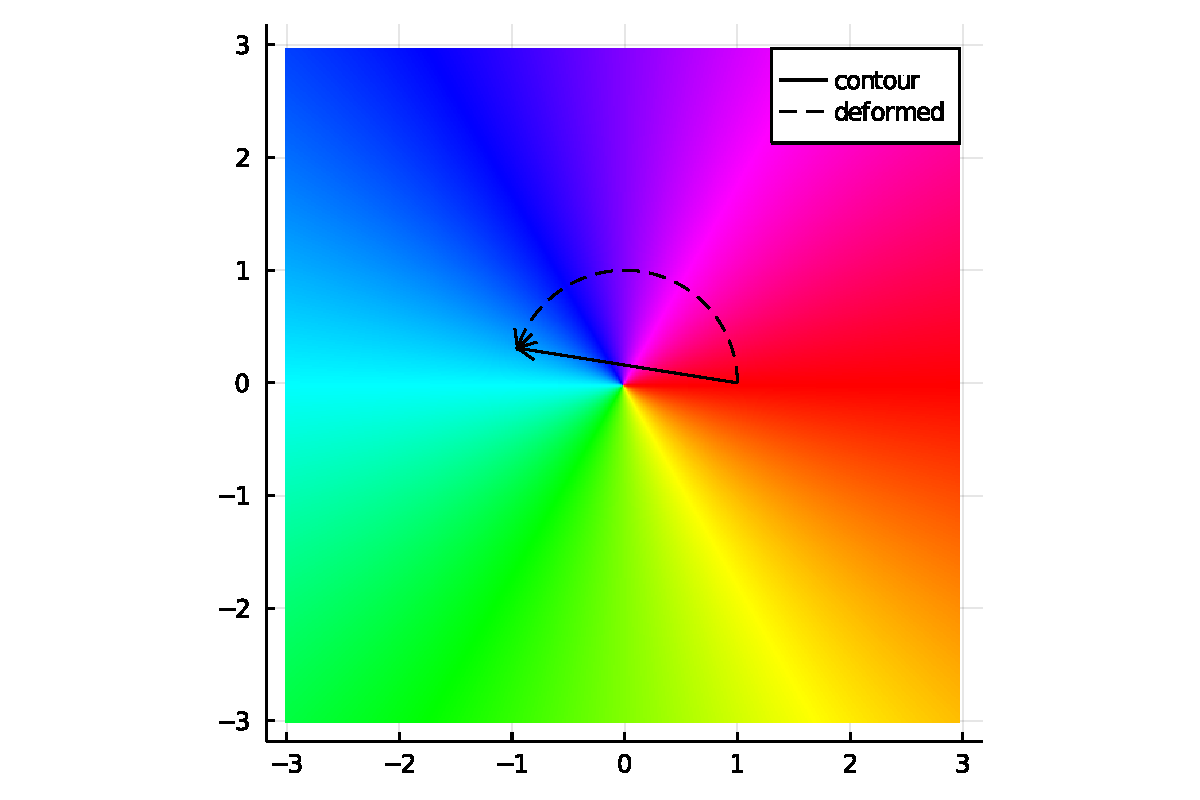
\includegraphics[width=0.6\linewidth]{C:/Users/mfaso/OneDrive/Documents/GitHub/M3M6AppliedComplexAnalysis/output/figures/Lecture10_3_1.pdf}}

This works all the way to the negative real axis. Thus we can calculate $\log_\pm (-1)$ using integrals over half circles:


\begin{lstlisting}
(*@\HLJLnf{plot}@*)(*@\HLJLp{(}@*)(*@\HLJLnf{Arc}@*)(*@\HLJLp{(}@*)(*@\HLJLnfB{0.}@*)(*@\HLJLp{,}@*)(*@\HLJLnfB{1.}@*)(*@\HLJLp{,(}@*)(*@\HLJLn{\ensuremath{\pi}}@*)(*@\HLJLp{,}@*)(*@\HLJLni{0}@*)(*@\HLJLp{));}@*) (*@\HLJLn{label}@*)(*@\HLJLoB{=}@*)(*@\HLJLs{"{}contour}@*) (*@\HLJLs{for}@*) (*@\HLJLs{log{\_}+"{}}@*)(*@\HLJLp{,}@*) (*@\HLJLn{arrow}@*)(*@\HLJLoB{=}@*)(*@\HLJLkc{true}@*)(*@\HLJLp{,}@*) (*@\HLJLn{ratio}@*)(*@\HLJLoB{=}@*)(*@\HLJLnfB{1.0}@*)(*@\HLJLp{)}@*)
(*@\HLJLnf{plot!}@*)(*@\HLJLp{(}@*)(*@\HLJLnf{Arc}@*)(*@\HLJLp{(}@*)(*@\HLJLnfB{0.}@*)(*@\HLJLp{,}@*)(*@\HLJLnfB{1.}@*)(*@\HLJLp{,(}@*)(*@\HLJLoB{-}@*)(*@\HLJLn{\ensuremath{\pi}}@*)(*@\HLJLp{,}@*)(*@\HLJLni{0}@*)(*@\HLJLp{));}@*) (*@\HLJLn{label}@*)(*@\HLJLoB{=}@*)(*@\HLJLs{"{}contour}@*) (*@\HLJLs{for}@*) (*@\HLJLs{log{\_}-"{}}@*)(*@\HLJLp{,}@*) (*@\HLJLn{arrow}@*)(*@\HLJLoB{=}@*)(*@\HLJLkc{true}@*)(*@\HLJLp{)}@*)
(*@\HLJLnf{scatter!}@*)(*@\HLJLp{([}@*)(*@\HLJLni{0}@*)(*@\HLJLp{],[}@*)(*@\HLJLni{0}@*)(*@\HLJLp{];}@*) (*@\HLJLn{label}@*)(*@\HLJLoB{=}@*)(*@\HLJLs{"{}pole}@*) (*@\HLJLs{in}@*) (*@\HLJLs{integrand"{}}@*)(*@\HLJLp{)}@*)
\end{lstlisting}

\cent{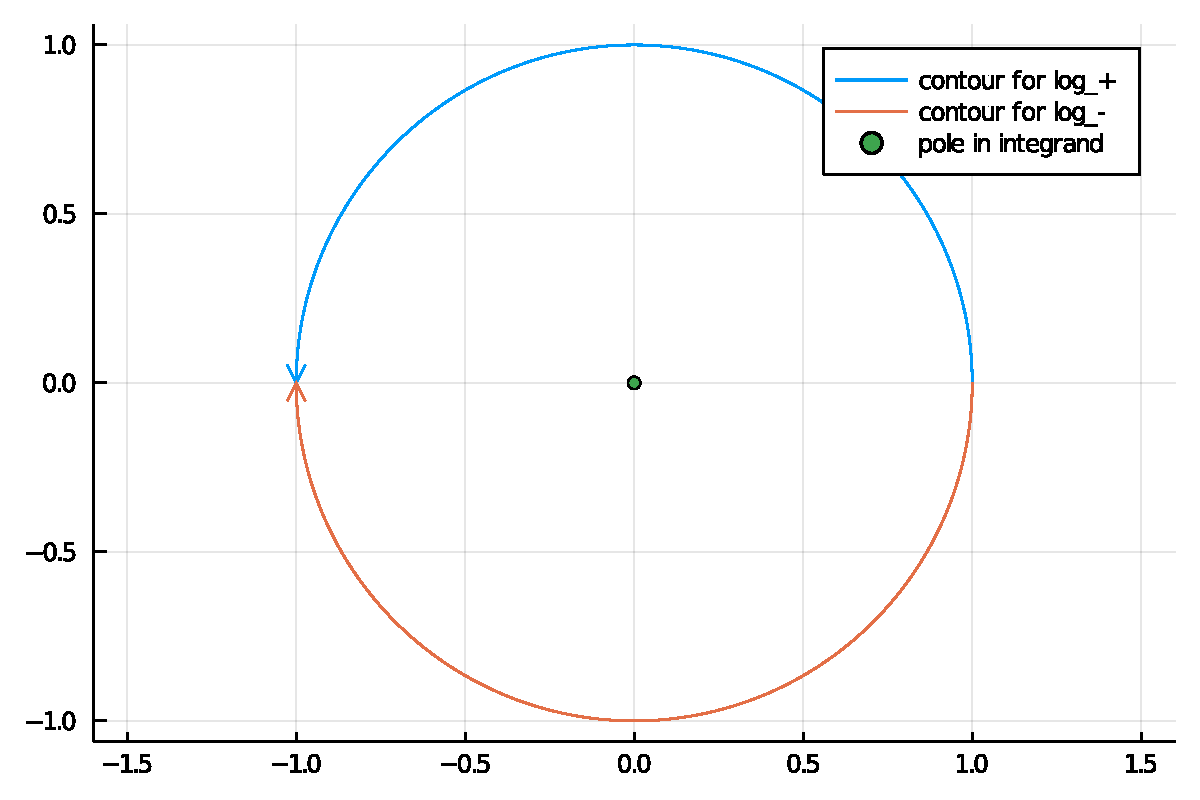
\includegraphics[width=0.6\linewidth]{C:/Users/mfaso/OneDrive/Documents/GitHub/M3M6AppliedComplexAnalysis/output/figures/Lecture10_4_1.pdf}}

Combining the two contours we have the \emph{subtractive jump} (for any $x < 0$)
\[
\log_+ x - \log_- x = \oint {\D\zeta \over \zeta}  = 2 \pi \I
\]
We can establish some properties. First we show that $\log z = - \log {1 \over z}$ by considering the change of variables $\zeta = {1 \over s}$.  Because $\gamma_z(t)^{-1}$ stays uniformly in the lower-half plane, we can deform it to a straight contour, which gives us the result:

\[
\log z = \int_{\gamma_z} {\D\zeta \over \zeta} = -\int_{{1 \over \zeta} \circ \gamma_z} {\D s \over s} = - \int_{\gamma_{z^{-1}}} {\D s \over s} = -\log z^{-1}
\]
Here's a plot of the relevant contours:


\begin{lstlisting}
(*@\HLJLnf{phaseplot}@*)(*@\HLJLp{(}@*)(*@\HLJLoB{-}@*)(*@\HLJLnfB{3..3}@*)(*@\HLJLp{,}@*) (*@\HLJLoB{-}@*)(*@\HLJLnfB{3..3}@*)(*@\HLJLp{,}@*) (*@\HLJLn{z}@*) (*@\HLJLoB{->}@*) (*@\HLJLnf{log}@*)(*@\HLJLp{(}@*)(*@\HLJLn{z}@*)(*@\HLJLp{))}@*)
(*@\HLJLn{z}@*) (*@\HLJLoB{=}@*) (*@\HLJLoB{-}@*)(*@\HLJLni{2}@*) (*@\HLJLoB{+}@*) (*@\HLJLni{2}@*)(*@\HLJLn{im}@*)
(*@\HLJLn{\ensuremath{\gamma}}@*) (*@\HLJLoB{=}@*) (*@\HLJLp{(}@*)(*@\HLJLn{z}@*)(*@\HLJLp{,}@*)(*@\HLJLn{t}@*)(*@\HLJLp{)}@*) (*@\HLJLoB{->}@*) (*@\HLJLni{1}@*) (*@\HLJLoB{+}@*) (*@\HLJLn{t}@*)(*@\HLJLoB{*}@*)(*@\HLJLp{(}@*)(*@\HLJLn{z}@*)(*@\HLJLoB{-}@*)(*@\HLJLni{1}@*)(*@\HLJLp{)}@*)
(*@\HLJLn{tt}@*) (*@\HLJLoB{=}@*) (*@\HLJLnf{range}@*)(*@\HLJLp{(}@*)(*@\HLJLni{0}@*)(*@\HLJLp{,}@*)(*@\HLJLn{stop}@*)(*@\HLJLoB{=}@*)(*@\HLJLni{1}@*)(*@\HLJLp{,}@*)(*@\HLJLn{length}@*)(*@\HLJLoB{=}@*)(*@\HLJLni{100}@*)(*@\HLJLp{)}@*)
(*@\HLJLnf{plot!}@*)(*@\HLJLp{(}@*)(*@\HLJLn{real}@*)(*@\HLJLoB{.}@*)(*@\HLJLp{(}@*)(*@\HLJLn{\ensuremath{\gamma}}@*)(*@\HLJLoB{.}@*)(*@\HLJLp{(}@*)(*@\HLJLn{z}@*)(*@\HLJLp{,}@*)(*@\HLJLn{tt}@*)(*@\HLJLp{)),}@*) (*@\HLJLn{imag}@*)(*@\HLJLoB{.}@*)(*@\HLJLp{(}@*)(*@\HLJLn{\ensuremath{\gamma}}@*)(*@\HLJLoB{.}@*)(*@\HLJLp{(}@*)(*@\HLJLn{z}@*)(*@\HLJLp{,}@*)(*@\HLJLn{tt}@*)(*@\HLJLp{));}@*) (*@\HLJLn{color}@*)(*@\HLJLoB{=:}@*)(*@\HLJLn{black}@*)(*@\HLJLp{,}@*) (*@\HLJLn{label}@*)(*@\HLJLoB{=}@*)(*@\HLJLs{"{}contour"{}}@*)(*@\HLJLp{,}@*) (*@\HLJLn{arrow}@*)(*@\HLJLoB{=}@*)(*@\HLJLkc{true}@*)(*@\HLJLp{)}@*)
(*@\HLJLnf{plot!}@*)(*@\HLJLp{(}@*)(*@\HLJLn{real}@*)(*@\HLJLoB{.}@*)(*@\HLJLp{(}@*)(*@\HLJLni{1}@*) (*@\HLJLoB{./}@*) (*@\HLJLn{\ensuremath{\gamma}}@*)(*@\HLJLoB{.}@*)(*@\HLJLp{(}@*)(*@\HLJLn{z}@*)(*@\HLJLp{,}@*)(*@\HLJLn{tt}@*)(*@\HLJLp{)),}@*) (*@\HLJLn{imag}@*)(*@\HLJLoB{.}@*)(*@\HLJLp{(}@*)(*@\HLJLni{1}@*) (*@\HLJLoB{./}@*) (*@\HLJLn{\ensuremath{\gamma}}@*)(*@\HLJLoB{.}@*)(*@\HLJLp{(}@*)(*@\HLJLn{z}@*)(*@\HLJLp{,}@*)(*@\HLJLn{tt}@*)(*@\HLJLp{));}@*) (*@\HLJLn{color}@*)(*@\HLJLoB{=:}@*)(*@\HLJLn{black}@*)(*@\HLJLp{,}@*) (*@\HLJLn{linestyle}@*)(*@\HLJLoB{=:}@*)(*@\HLJLn{dash}@*)(*@\HLJLp{,}@*) (*@\HLJLn{arrow}@*)(*@\HLJLoB{=}@*)(*@\HLJLkc{true}@*)(*@\HLJLp{,}@*) (*@\HLJLn{label}@*)(*@\HLJLoB{=}@*)(*@\HLJLs{"{}change}@*) (*@\HLJLs{of}@*) (*@\HLJLs{variables}@*) (*@\HLJLs{contour"{}}@*)(*@\HLJLp{)}@*)
(*@\HLJLnf{plot!}@*)(*@\HLJLp{(}@*)(*@\HLJLn{real}@*)(*@\HLJLoB{.}@*)(*@\HLJLp{(}@*)(*@\HLJLn{\ensuremath{\gamma}}@*)(*@\HLJLoB{.}@*)(*@\HLJLp{(}@*)(*@\HLJLni{1}@*)(*@\HLJLoB{/}@*)(*@\HLJLn{z}@*)(*@\HLJLp{,}@*)(*@\HLJLn{tt}@*)(*@\HLJLp{)),}@*) (*@\HLJLn{imag}@*)(*@\HLJLoB{.}@*)(*@\HLJLp{(}@*)(*@\HLJLn{\ensuremath{\gamma}}@*)(*@\HLJLoB{.}@*)(*@\HLJLp{(}@*)(*@\HLJLni{1}@*)(*@\HLJLoB{/}@*)(*@\HLJLn{z}@*)(*@\HLJLp{,}@*)(*@\HLJLn{tt}@*)(*@\HLJLp{));}@*) (*@\HLJLn{color}@*)(*@\HLJLoB{=:}@*)(*@\HLJLn{black}@*)(*@\HLJLp{,}@*) (*@\HLJLn{linestyle}@*)(*@\HLJLoB{=:}@*)(*@\HLJLn{dashdot}@*)(*@\HLJLp{,}@*) (*@\HLJLn{arrow}@*)(*@\HLJLoB{=}@*)(*@\HLJLkc{true}@*)(*@\HLJLp{,}@*) (*@\HLJLn{label}@*)(*@\HLJLoB{=}@*)(*@\HLJLs{"{}deformed}@*) (*@\HLJLs{contour"{}}@*)(*@\HLJLp{)}@*)
\end{lstlisting}

Here we see by looking at the phase plot that the two functions match:
\begin{lstlisting}
(*@\HLJLnf{phaseplot}@*)(*@\HLJLp{(}@*)(*@\HLJLoB{-}@*)(*@\HLJLnfB{3..3}@*)(*@\HLJLp{,}@*) (*@\HLJLoB{-}@*)(*@\HLJLnfB{3..3}@*)(*@\HLJLp{,}@*) (*@\HLJLn{z}@*) (*@\HLJLoB{->}@*) (*@\HLJLoB{-}@*)(*@\HLJLnf{log}@*)(*@\HLJLp{(}@*)(*@\HLJLni{1}@*)(*@\HLJLoB{/}@*)(*@\HLJLn{z}@*)(*@\HLJLp{))}@*)
\end{lstlisting}


\hspace*{-3.75cm}\mbox{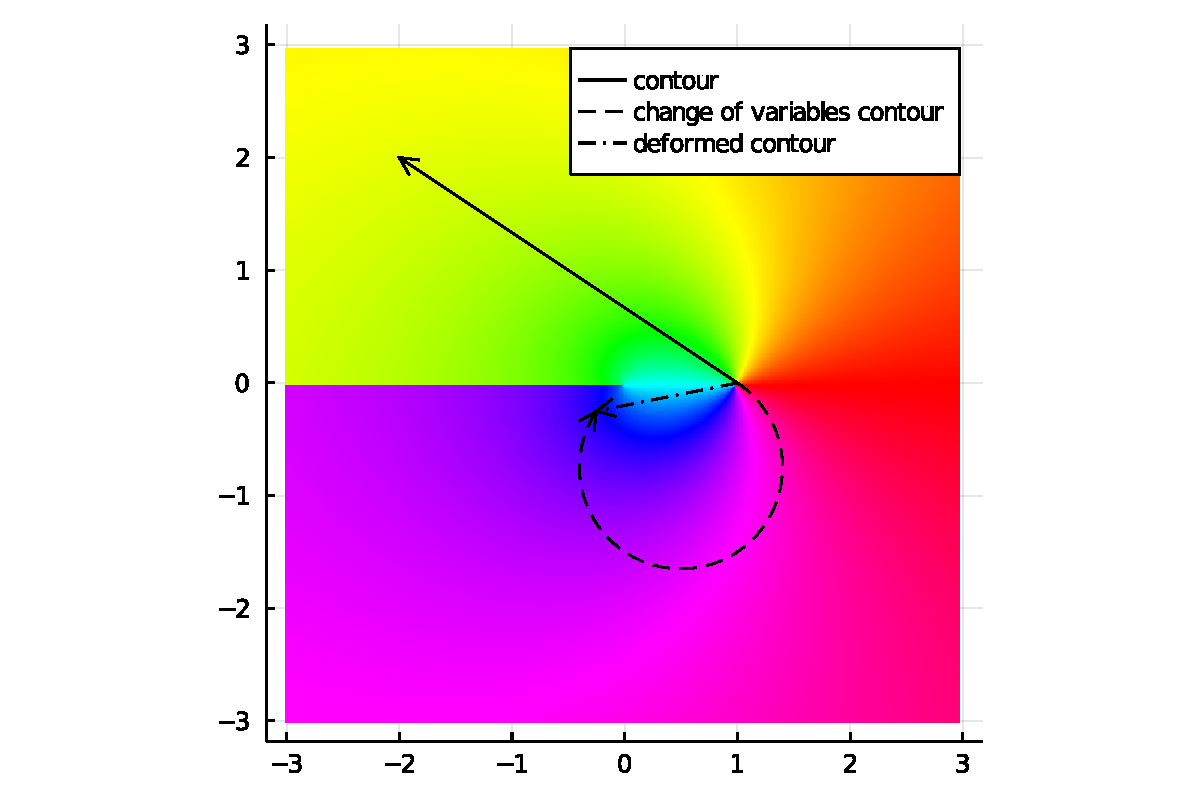
\includegraphics[width=0.7\linewidth]{C:/Users/mfaso/OneDrive/Documents/GitHub/M3M6AppliedComplexAnalysis/output/figures/Lecture10_5_1.pdf}
\hspace*{-3.75cm}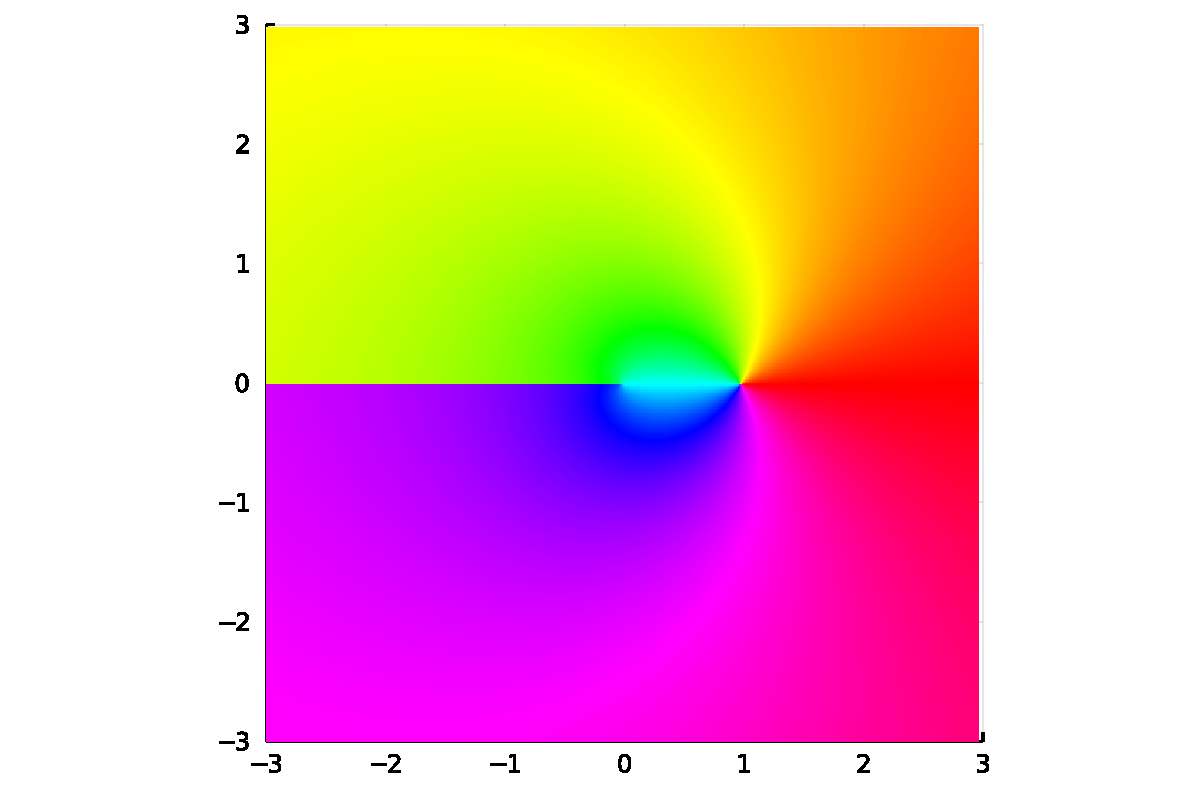
\includegraphics[width=0.7\linewidth]{C:/Users/mfaso/OneDrive/Documents/GitHub/M3M6AppliedComplexAnalysis/output/figures/Lecture10_6_1.pdf}}
%\cent{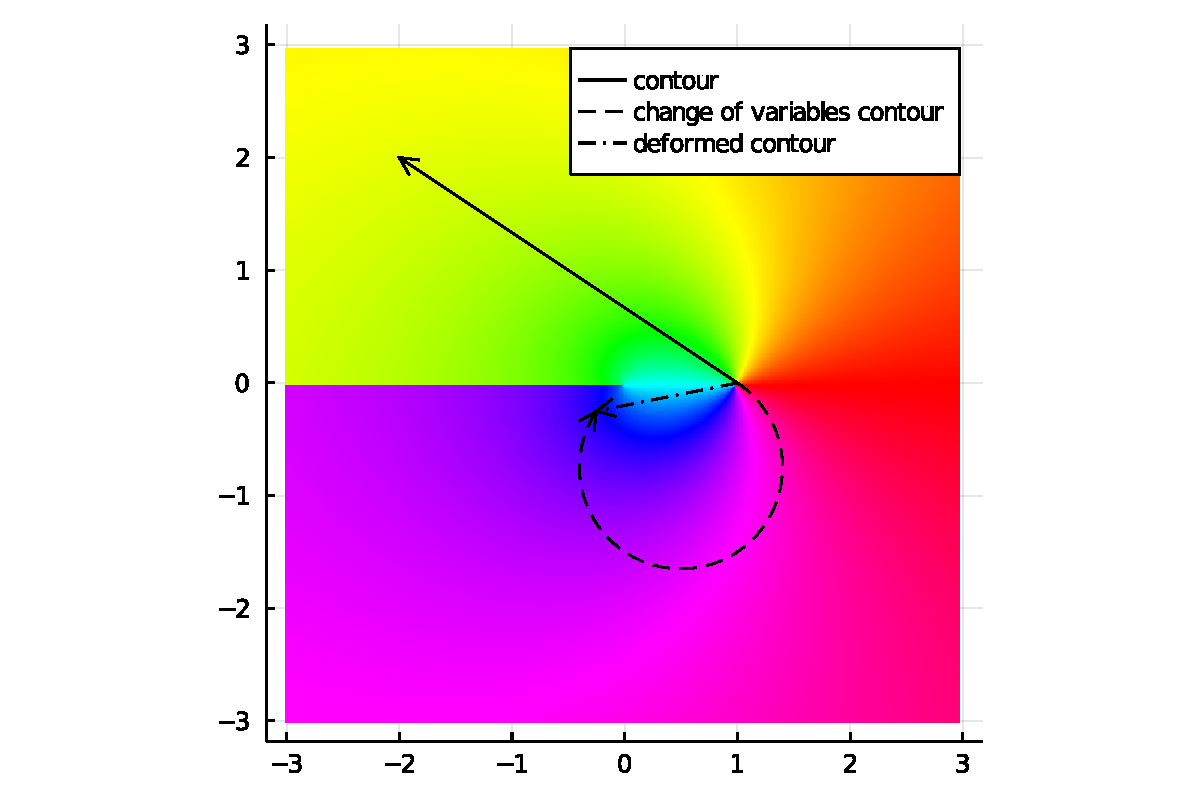
\includegraphics[width=0.58\linewidth]{C:/Users/mfaso/OneDrive/Documents/GitHub/M3M6AppliedComplexAnalysis/output/figures/Lecture10_5_1.pdf}\\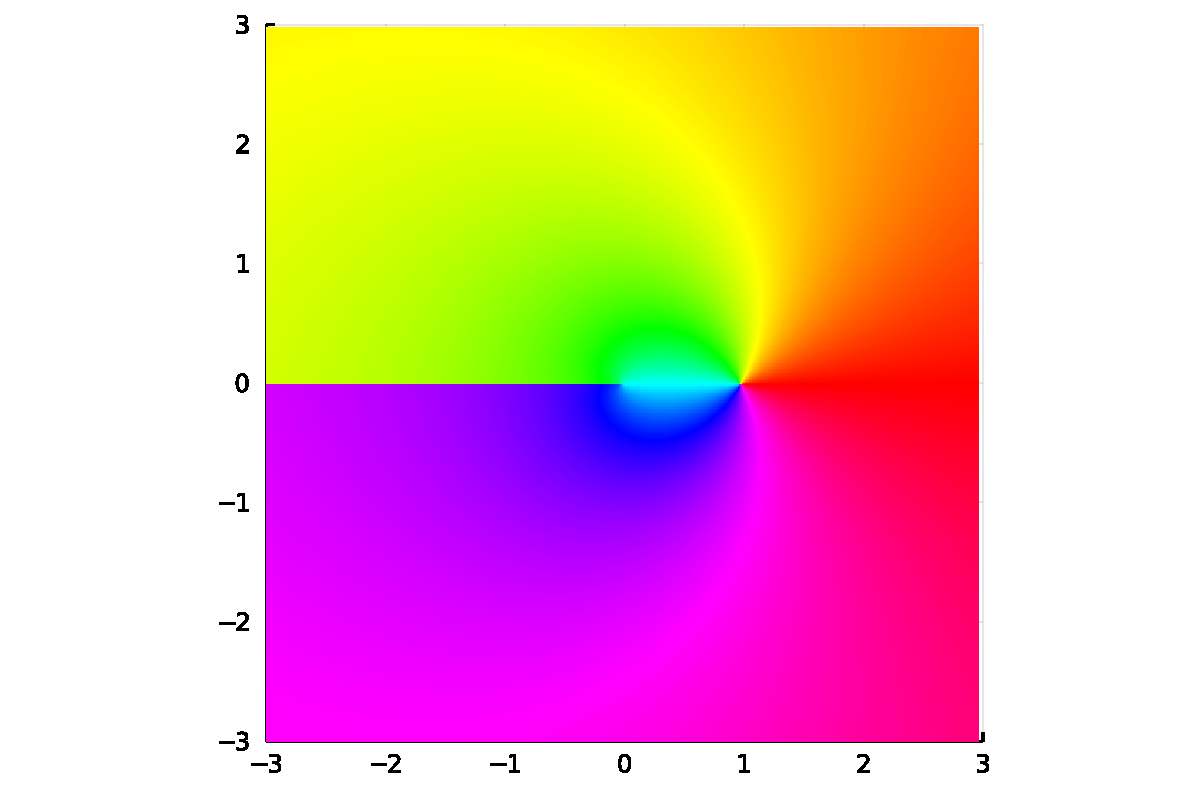
\includegraphics[width=0.58\linewidth]{C:/Users/mfaso/OneDrive/Documents/GitHub/M3M6AppliedComplexAnalysis/output/figures/Lecture10_6_1.pdf}}
\newpage
\subsection{Algebraic powers}
We define algebraic powers in terms of logarithms, which gives us what we need to know about their jumps.

\textbf{Definition (algebraic power)}

\[
z^\alpha := \E^{\alpha \log z}
\]
Note, for example, when $\alpha = 1/2$, $\sqrt z \equiv z^{1/2}$ is only one solution to $y^2 = z$.

Here are phase plots showing that $\sqrt{z}$ also has a branch cut on $(-\infty,0]$ on both of its branches:


\begin{lstlisting}
(*@\HLJLn{\ensuremath{\alpha}}@*) (*@\HLJLoB{=}@*) (*@\HLJLnfB{0.5}@*)
(*@\HLJLnf{phaseplot}@*)(*@\HLJLp{(}@*)(*@\HLJLoB{-}@*)(*@\HLJLnfB{3..3}@*)(*@\HLJLp{,}@*) (*@\HLJLoB{-}@*)(*@\HLJLnfB{3..3}@*)(*@\HLJLp{,}@*) (*@\HLJLn{z}@*) (*@\HLJLoB{->}@*) (*@\HLJLn{z}@*)(*@\HLJLoB{{\textasciicircum}}@*)(*@\HLJLn{\ensuremath{\alpha}}@*)(*@\HLJLp{)}@*)
\end{lstlisting}

\begin{lstlisting}
(*@\HLJLnf{phaseplot}@*)(*@\HLJLp{(}@*)(*@\HLJLoB{-}@*)(*@\HLJLnfB{3..3}@*)(*@\HLJLp{,}@*) (*@\HLJLoB{-}@*)(*@\HLJLnfB{3..3}@*)(*@\HLJLp{,}@*) (*@\HLJLn{z}@*) (*@\HLJLoB{->}@*) (*@\HLJLoB{-}@*)(*@\HLJLn{z}@*)(*@\HLJLoB{{\textasciicircum}}@*)(*@\HLJLn{\ensuremath{\alpha}}@*)(*@\HLJLp{)}@*)
\end{lstlisting}


\mbox{\hspace*{-3.75cm}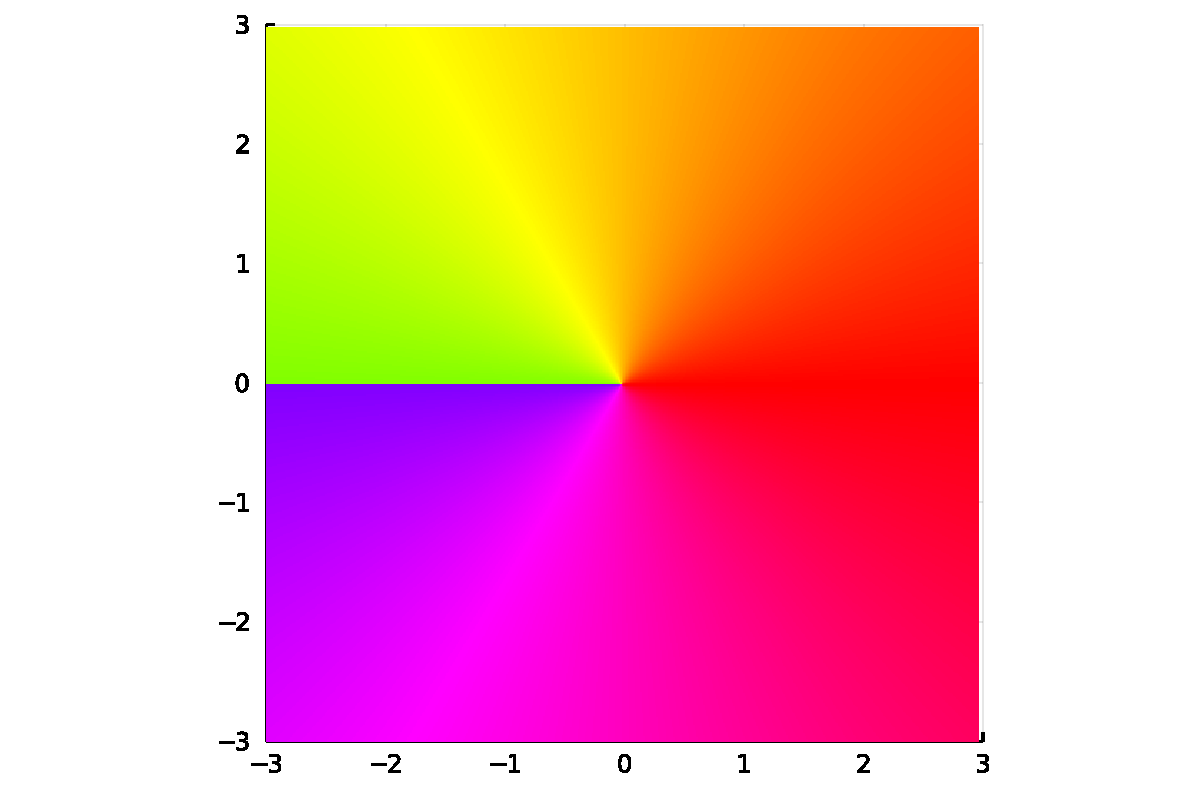
\includegraphics[width=0.7\linewidth]{C:/Users/mfaso/OneDrive/Documents/GitHub/M3M6AppliedComplexAnalysis/output/figures/Lecture10_7_1.pdf}\hspace*{-3.75cm}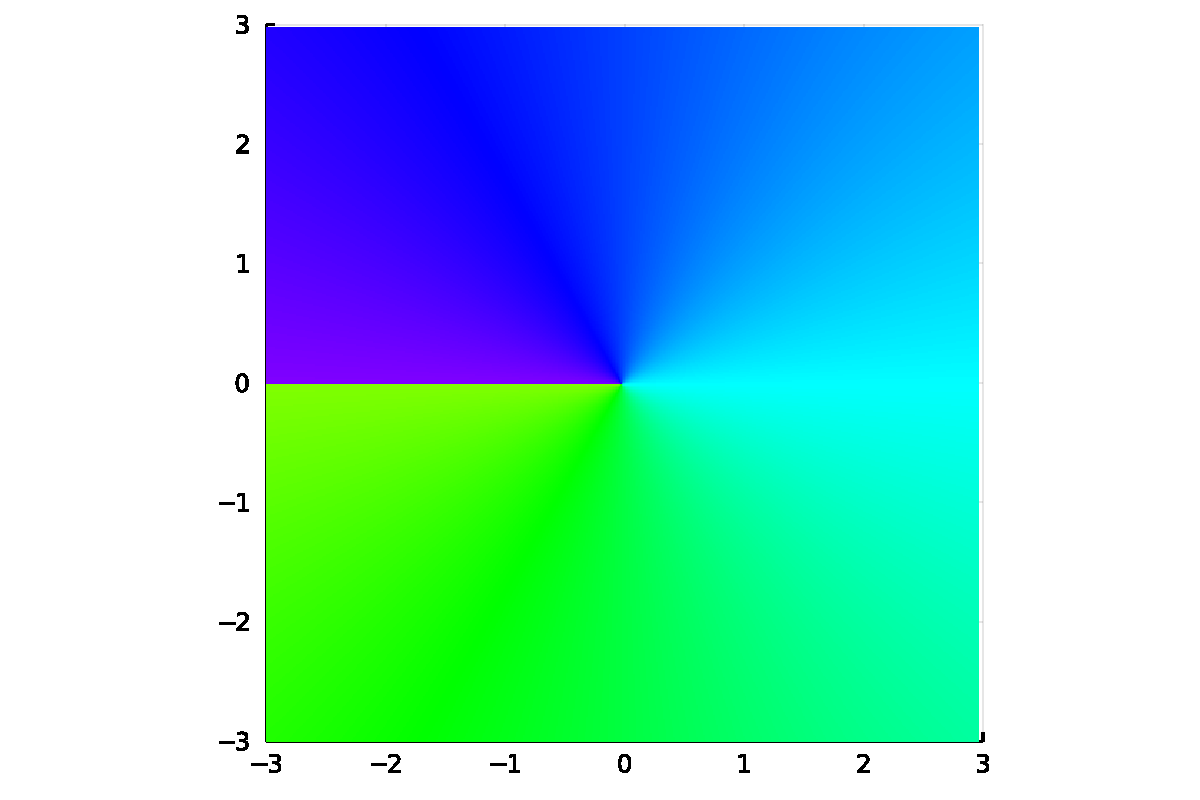
\includegraphics[width=0.7\linewidth]{C:/Users/mfaso/OneDrive/Documents/GitHub/M3M6AppliedComplexAnalysis/output/figures/Lecture10_8_1.pdf}}
\newpage
On the branch cut  along $(-\infty,0]$ it has the jump:

\[
{x_+^\alpha \over x_-^\alpha} = \E^{\alpha (\log_+ x - \log_- x)} = \E^{2 \pi \I \alpha}
\]
In particular,

\[
\sqrt{x}_+ = -\sqrt{x}_- = i \sqrt{|x|}
\]
These are \emph{multiplicative jumps}. We also have a \emph{subtractive jump}:


\begin{align*}
x_+^\alpha - x_-^\alpha &= \E^{\alpha \log_+ x} - \E^{\alpha \log_- x} = \E^{\alpha \log(-x) + \I  \pi \alpha} - \E^{\alpha \log(-x) - \I \pi \alpha} \cr
    & = 2 \I (-x)^\alpha \sin \pi \alpha
\end{align*}
and an \emph{additive jump}:


\begin{align*}
x_+^\alpha + x_-^\alpha & = 2  (-x)^\alpha \cos \pi \alpha
\end{align*}
In particular, for $x < 0$,


\begin{align*}
\sqrt{x}_+ - \sqrt{x}_- &= 2 \I \sqrt{-x} \\
\sqrt{x}_+ + \sqrt{x}_- &= 0
\end{align*}
Let's look at another example: $\varphi(z) = \sqrt{z-1}\sqrt{z+1}$. Each square root term induces a jump: one on $(-\infty,-1]$ and one on $(-\infty,1]$. Surprisingly these jumps cancel out, in fact (as we explain below) $\varphi$ is analytic off $[-1,1]$, as can be seen from the phase portrait:


\begin{lstlisting}
(*@\HLJLn{\ensuremath{\varphi}}@*) (*@\HLJLoB{=}@*) (*@\HLJLn{z}@*) (*@\HLJLoB{->}@*) (*@\HLJLnf{sqrt}@*)(*@\HLJLp{(}@*)(*@\HLJLn{z}@*)(*@\HLJLoB{-}@*)(*@\HLJLni{1}@*)(*@\HLJLp{)}@*)(*@\HLJLoB{*}@*)(*@\HLJLnf{sqrt}@*)(*@\HLJLp{(}@*)(*@\HLJLn{z}@*)(*@\HLJLoB{+}@*)(*@\HLJLni{1}@*)(*@\HLJLp{)}@*)
(*@\HLJLnf{phaseplot}@*)(*@\HLJLp{(}@*)(*@\HLJLoB{-}@*)(*@\HLJLnfB{3..3}@*)(*@\HLJLp{,}@*) (*@\HLJLoB{-}@*)(*@\HLJLnfB{3..3}@*)(*@\HLJLp{,}@*) (*@\HLJLn{\ensuremath{\varphi}}@*)(*@\HLJLp{)}@*)
\end{lstlisting}

\cent{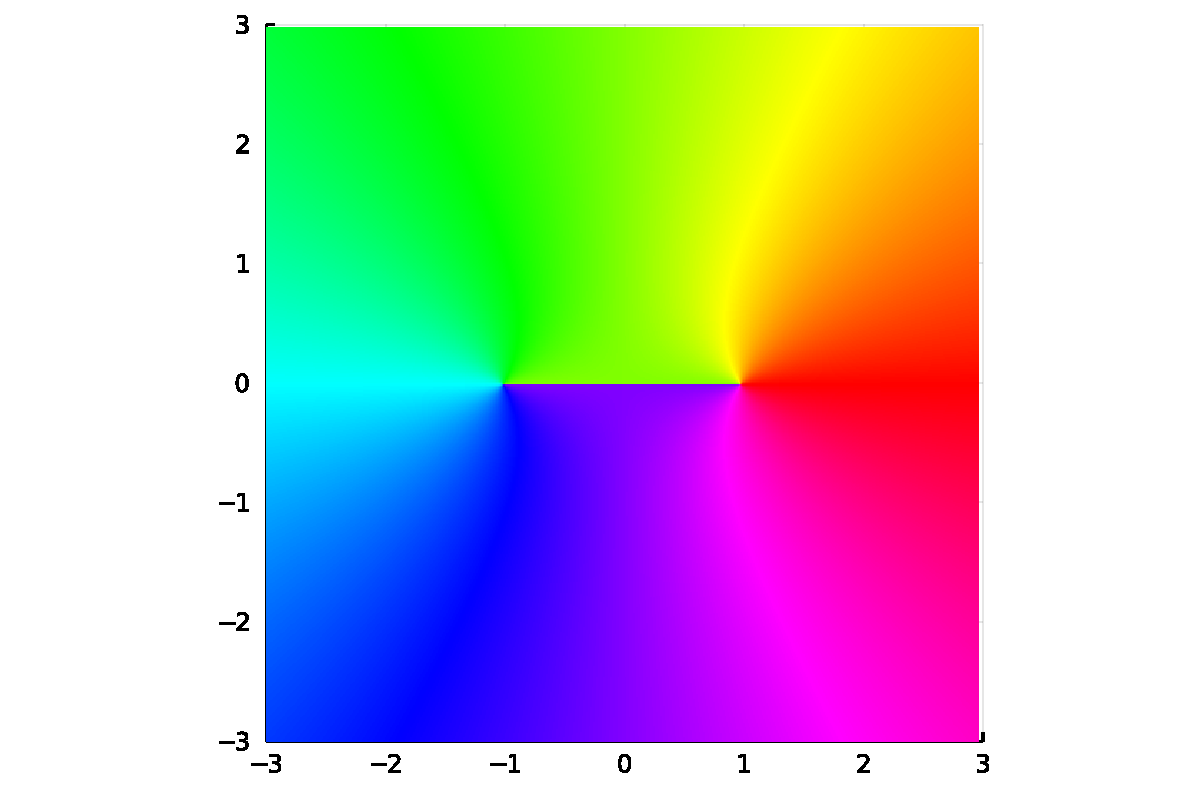
\includegraphics[width=0.8\linewidth]{C:/Users/mfaso/OneDrive/Documents/GitHub/M3M6AppliedComplexAnalysis/output/figures/Lecture10_9_1.pdf}}

For $-1 < x < 1$ we have the multiplicative jump:

\[
\varphi_+(x) = \sqrt{x-1}_+ \sqrt{x+1} = - \sqrt{x-1}_- \sqrt{x+1} = -\varphi_-(x)
\]
which gives the additive jump

\[
\varphi_+(x) + \varphi_-(x) = 0
\]
But we also have a \emph{subtractive jump}:

\[
\varphi_+(x) - \varphi_-(x) = (\sqrt{x-1}_+ - \sqrt{x-1}_-) \sqrt{x+1} = 2\I \sqrt{1-x}\sqrt{x+1} = 2\I \sqrt{1 - x^2}
\]
For $x < -1$ we actually have continuity:

\[
\varphi_+(x) = \sqrt{x-1}_+ \sqrt{x+1}_+ = (- \sqrt{x-1}_-)(- \sqrt{x+1}_-) = \varphi_-(x)
\]
This feature is what we use to show analyticity.
\newpage

\section{Inferred analyticity}
Here we review properties of inferring analyticity from continuity.

\textbf{Theorem (continuity on a curve implies analyticity)} Let $D$ be a domain and $\gamma \subset D$ a contour. Suppose $f$ is analytic in $D \backslash \gamma$, and continuous on the interior of $\gamma$. Then $f$ is analytic in $D \backslash \{\gamma(a), \gamma(b) \}$.

\textbf{Sketch of Proof}

For simplicity, suppose $D$ is a circle of radius 2 and $\gamma$ is the interval $[-1,1]$. For any $z$ off the interval, we can write

\[
f(z) = {1 \over 2 \pi \I} \oint_{\Gamma_x} {f(\zeta) \over  \zeta - z} \D\zeta
\]
where $\Gamma_x$ is a simple closed contour that surrounds $z$ and passes through $x$ in both directions:


\begin{lstlisting}
(*@\HLJLn{z}@*) (*@\HLJLoB{=}@*) (*@\HLJLnfB{0.2}@*)(*@\HLJLoB{+}@*)(*@\HLJLnfB{0.2}@*)(*@\HLJLn{im}@*)
(*@\HLJLn{x}@*) (*@\HLJLoB{=}@*) (*@\HLJLnfB{0.1}@*)
(*@\HLJLn{\ensuremath{\varepsilon}}@*) (*@\HLJLoB{=}@*) (*@\HLJLnfB{0.001}@*)
(*@\HLJLnf{scatter}@*)(*@\HLJLp{([}@*)(*@\HLJLn{x}@*)(*@\HLJLp{],[}@*)(*@\HLJLnfB{0.}@*)(*@\HLJLp{];}@*) (*@\HLJLn{label}@*)(*@\HLJLoB{=}@*)(*@\HLJLs{"{}x"{}}@*)(*@\HLJLp{,}@*) (*@\HLJLn{xlims}@*)(*@\HLJLoB{=}@*)(*@\HLJLp{(}@*)(*@\HLJLoB{-}@*)(*@\HLJLnfB{1.5}@*)(*@\HLJLp{,}@*)(*@\HLJLnfB{1.5}@*)(*@\HLJLp{),}@*) (*@\HLJLn{ylims}@*)(*@\HLJLoB{=}@*)(*@\HLJLp{(}@*)(*@\HLJLoB{-}@*)(*@\HLJLnfB{0.5}@*)(*@\HLJLp{,}@*)(*@\HLJLnfB{0.5}@*)(*@\HLJLp{),}@*)(*@\HLJLn{ratio}@*)(*@\HLJLoB{=}@*)(*@\HLJLnfB{1.0}@*)(*@\HLJLp{)}@*)
(*@\HLJLnf{scatter!}@*)(*@\HLJLp{([}@*)(*@\HLJLnf{real}@*)(*@\HLJLp{(}@*)(*@\HLJLn{z}@*)(*@\HLJLp{)],[}@*)(*@\HLJLnf{imag}@*)(*@\HLJLp{(}@*)(*@\HLJLn{z}@*)(*@\HLJLp{)];}@*) (*@\HLJLn{label}@*)(*@\HLJLoB{=}@*)(*@\HLJLs{"{}z"{}}@*)(*@\HLJLp{)}@*)
(*@\HLJLnf{plot!}@*)(*@\HLJLp{(}@*)(*@\HLJLoB{-}@*)(*@\HLJLnfB{1..1}@*)(*@\HLJLp{;}@*) (*@\HLJLn{label}@*)(*@\HLJLoB{=}@*)(*@\HLJLs{"{}Unit}@*) (*@\HLJLs{interval"{}}@*)(*@\HLJLp{,}@*) (*@\HLJLn{linestyle}@*)(*@\HLJLoB{=:}@*)(*@\HLJLn{dot}@*)(*@\HLJLp{)}@*)
(*@\HLJLn{\ensuremath{\Gamma}{\_}x}@*) (*@\HLJLoB{=}@*)  (*@\HLJLnf{Arc}@*)(*@\HLJLp{(}@*)(*@\HLJLn{z}@*)(*@\HLJLp{,}@*) (*@\HLJLnfB{0.1}@*)(*@\HLJLp{,}@*) (*@\HLJLp{(}@*)(*@\HLJLoB{-}@*)(*@\HLJLn{\ensuremath{\pi}}@*)(*@\HLJLoB{/}@*)(*@\HLJLni{2}@*)(*@\HLJLp{,}@*)(*@\HLJLn{\ensuremath{\pi}}@*)(*@\HLJLp{))}@*) (*@\HLJLoB{\ensuremath{\cup}}@*) (*@\HLJLnf{Segment}@*)(*@\HLJLp{(}@*)(*@\HLJLnfB{0.2}@*)(*@\HLJLoB{+}@*)(*@\HLJLnfB{0.1}@*)(*@\HLJLn{im}@*)(*@\HLJLp{,}@*)(*@\HLJLnfB{0.2}@*) (*@\HLJLoB{+}@*)(*@\HLJLnfB{0.0}@*)(*@\HLJLn{im}@*)(*@\HLJLp{)}@*) (*@\HLJLoB{\ensuremath{\cup}}@*) (*@\HLJLnf{Segment}@*)(*@\HLJLp{(}@*)(*@\HLJLnfB{0.2}@*)  (*@\HLJLoB{+}@*)(*@\HLJLnfB{0.0}@*)(*@\HLJLn{im}@*)(*@\HLJLp{,}@*) (*@\HLJLoB{-}@*)(*@\HLJLnfB{0.9}@*) (*@\HLJLoB{+}@*)(*@\HLJLnfB{0.0}@*)(*@\HLJLn{im}@*)(*@\HLJLp{)}@*) (*@\HLJLoB{\ensuremath{\cup}}@*)
     (*@\HLJLnf{Circle}@*)(*@\HLJLp{(}@*)(*@\HLJLoB{-}@*)(*@\HLJLnfB{1.0}@*)(*@\HLJLp{,}@*) (*@\HLJLnfB{0.1}@*)(*@\HLJLp{)}@*) (*@\HLJLoB{\ensuremath{\cup}}@*) (*@\HLJLnf{Segment}@*)(*@\HLJLp{(}@*)(*@\HLJLoB{-}@*)(*@\HLJLnfB{0.9}@*) (*@\HLJLoB{-}@*)(*@\HLJLnfB{0.0}@*)(*@\HLJLn{im}@*)(*@\HLJLp{,}@*) (*@\HLJLnfB{0.2}@*)  (*@\HLJLoB{-}@*)(*@\HLJLnfB{0.0}@*)(*@\HLJLn{im}@*)(*@\HLJLp{)}@*) (*@\HLJLoB{\ensuremath{\cup}}@*) (*@\HLJLnf{Segment}@*)(*@\HLJLp{(}@*)(*@\HLJLnfB{0.2}@*)(*@\HLJLoB{-}@*)(*@\HLJLnfB{0.0}@*)(*@\HLJLn{im}@*)(*@\HLJLp{,}@*) (*@\HLJLnfB{0.2}@*) (*@\HLJLoB{-}@*) (*@\HLJLnfB{0.2}@*)(*@\HLJLn{im}@*)(*@\HLJLp{)}@*) (*@\HLJLoB{\ensuremath{\cup}}@*)
      (*@\HLJLnf{Segment}@*)(*@\HLJLp{(}@*)(*@\HLJLnfB{0.2}@*) (*@\HLJLoB{-}@*) (*@\HLJLnfB{0.2}@*)(*@\HLJLn{im}@*)(*@\HLJLp{,}@*) (*@\HLJLoB{-}@*)(*@\HLJLnfB{1.2}@*)(*@\HLJLoB{-}@*)(*@\HLJLnfB{0.2}@*)(*@\HLJLn{im}@*)(*@\HLJLp{)}@*) (*@\HLJLoB{\ensuremath{\cup}}@*) (*@\HLJLnf{Segment}@*)(*@\HLJLp{(}@*)(*@\HLJLoB{-}@*)(*@\HLJLnfB{1.2}@*) (*@\HLJLoB{-}@*)(*@\HLJLnfB{0.2}@*)(*@\HLJLn{im}@*)(*@\HLJLp{,}@*) (*@\HLJLoB{-}@*)(*@\HLJLnfB{1.2}@*)(*@\HLJLoB{+}@*) (*@\HLJLnfB{0.2}@*)(*@\HLJLn{im}@*)(*@\HLJLp{)}@*) (*@\HLJLoB{\ensuremath{\cup}}@*)
        (*@\HLJLnf{Segment}@*)(*@\HLJLp{(}@*)(*@\HLJLoB{-}@*)(*@\HLJLnfB{1.2}@*)(*@\HLJLoB{+}@*) (*@\HLJLnfB{0.2}@*)(*@\HLJLn{im}@*)(*@\HLJLp{,}@*) (*@\HLJLnfB{0.1}@*)(*@\HLJLoB{+}@*)(*@\HLJLnfB{0.2}@*)(*@\HLJLn{im}@*)(*@\HLJLp{)}@*)
(*@\HLJLnf{plot!}@*)(*@\HLJLp{(}@*)(*@\HLJLn{\ensuremath{\Gamma}{\_}x}@*)(*@\HLJLp{;}@*) (*@\HLJLn{label}@*)(*@\HLJLoB{=}@*)(*@\HLJLs{"{}Contour"{}}@*)(*@\HLJLp{)}@*)
\end{lstlisting}
\cent{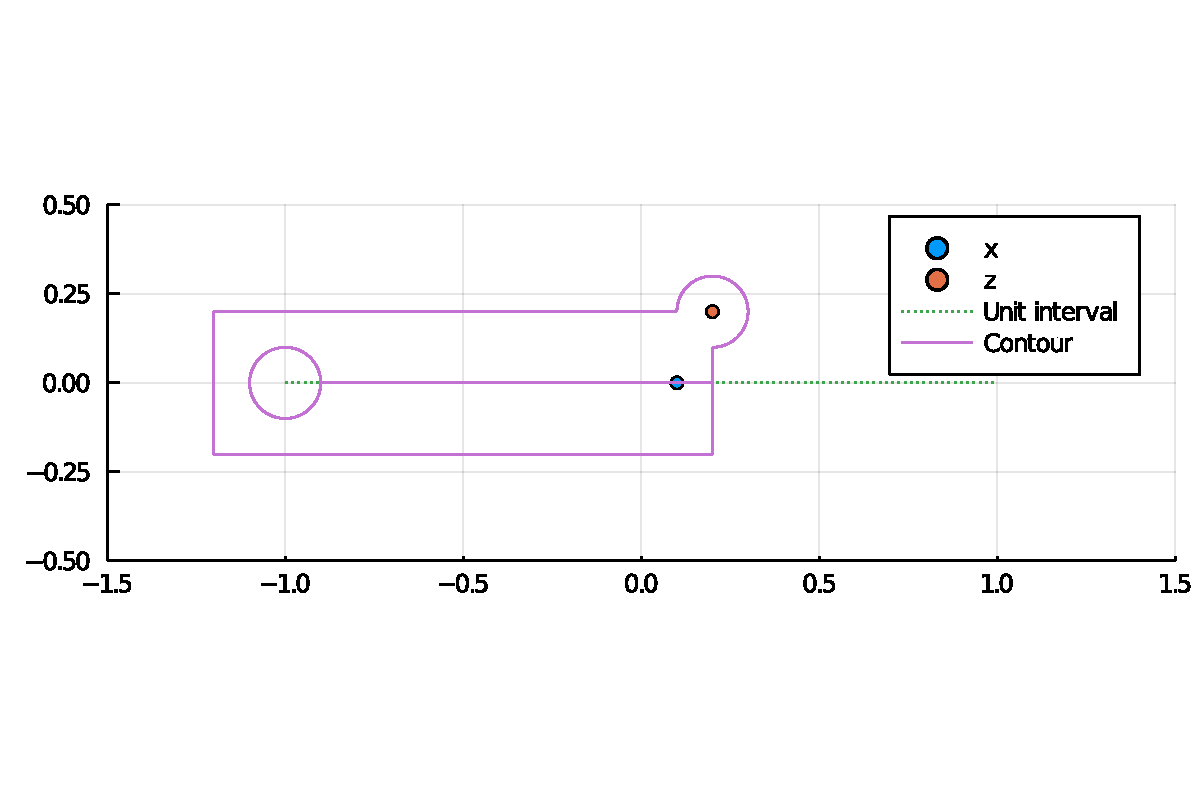
\includegraphics[width=0.8\linewidth]{C:/Users/mfaso/OneDrive/Documents/GitHub/M3M6AppliedComplexAnalysis/output/figures/Lecture10_10_1.pdf}}

Because $f$ is continuous at $x$, we have

\[
f_+(x) = f_-(x) = f(x)
\]
where

\[
f_\pm(x) = \lim_{\epsilon \rightarrow 0} f(x \pm \I \epsilon)
\]
Therefore, the two integrals along $[-1,1]$ cancel out and we get:

\[
    f(z) = {1 \over 2 \pi \I} \oint_{{\tilde \Gamma}_x} {f(\zeta) \over \zeta - z} \D \zeta
\]
where ${\tilde \Gamma}_x$ is $\Gamma_x$ with the contour on the interval removed:


\begin{lstlisting}
(*@\HLJLn{z}@*) (*@\HLJLoB{=}@*) (*@\HLJLnfB{0.2}@*)(*@\HLJLoB{+}@*)(*@\HLJLnfB{0.2}@*)(*@\HLJLn{im}@*)
(*@\HLJLn{x}@*) (*@\HLJLoB{=}@*) (*@\HLJLnfB{0.1}@*)
(*@\HLJLnf{scatter}@*)(*@\HLJLp{([}@*)(*@\HLJLn{x}@*)(*@\HLJLp{],[}@*)(*@\HLJLnfB{0.}@*)(*@\HLJLp{];}@*) (*@\HLJLn{label}@*)(*@\HLJLoB{=}@*)(*@\HLJLs{"{}x"{}}@*)(*@\HLJLp{,}@*) (*@\HLJLn{xlims}@*)(*@\HLJLoB{=}@*)(*@\HLJLp{(}@*)(*@\HLJLoB{-}@*)(*@\HLJLnfB{1.5}@*)(*@\HLJLp{,}@*)(*@\HLJLnfB{1.5}@*)(*@\HLJLp{),}@*) (*@\HLJLn{ylims}@*)(*@\HLJLoB{=}@*)(*@\HLJLp{(}@*)(*@\HLJLoB{-}@*)(*@\HLJLnfB{0.5}@*)(*@\HLJLp{,}@*)(*@\HLJLnfB{0.5}@*)(*@\HLJLp{),}@*)(*@\HLJLn{ratio}@*)(*@\HLJLoB{=}@*)(*@\HLJLnfB{1.0}@*)(*@\HLJLp{)}@*)
(*@\HLJLnf{scatter!}@*)(*@\HLJLp{([}@*)(*@\HLJLnf{real}@*)(*@\HLJLp{(}@*)(*@\HLJLn{z}@*)(*@\HLJLp{)],[}@*)(*@\HLJLnf{imag}@*)(*@\HLJLp{(}@*)(*@\HLJLn{z}@*)(*@\HLJLp{)];}@*) (*@\HLJLn{label}@*)(*@\HLJLoB{=}@*)(*@\HLJLs{"{}z"{}}@*)(*@\HLJLp{)}@*)
(*@\HLJLnf{plot!}@*)(*@\HLJLp{(}@*)(*@\HLJLoB{-}@*)(*@\HLJLnfB{1..1}@*)(*@\HLJLp{;}@*) (*@\HLJLn{label}@*)(*@\HLJLoB{=}@*)(*@\HLJLs{"{}Unit}@*) (*@\HLJLs{interval"{}}@*)(*@\HLJLp{,}@*) (*@\HLJLn{linestyle}@*)(*@\HLJLoB{=:}@*)(*@\HLJLn{dot}@*)(*@\HLJLp{)}@*)
(*@\HLJLn{\ensuremath{\Gamma}t{\_}x}@*) (*@\HLJLoB{=}@*)  (*@\HLJLnf{Arc}@*)(*@\HLJLp{(}@*)(*@\HLJLn{z}@*)(*@\HLJLp{,}@*) (*@\HLJLnfB{0.1}@*)(*@\HLJLp{,}@*) (*@\HLJLp{(}@*)(*@\HLJLoB{-}@*)(*@\HLJLn{\ensuremath{\pi}}@*)(*@\HLJLoB{/}@*)(*@\HLJLni{2}@*)(*@\HLJLp{,}@*)(*@\HLJLn{\ensuremath{\pi}}@*)(*@\HLJLp{))}@*) (*@\HLJLoB{\ensuremath{\cup}}@*) (*@\HLJLnf{Segment}@*)(*@\HLJLp{(}@*)(*@\HLJLnfB{0.2}@*)(*@\HLJLoB{+}@*)(*@\HLJLnfB{0.1}@*)(*@\HLJLn{im}@*)(*@\HLJLp{,}@*)(*@\HLJLnfB{0.2}@*) (*@\HLJLoB{-}@*)(*@\HLJLnfB{0.2}@*)(*@\HLJLn{im}@*)(*@\HLJLp{)}@*) (*@\HLJLoB{\ensuremath{\cup}}@*)    (*@\HLJLnf{Circle}@*)(*@\HLJLp{(}@*)(*@\HLJLoB{-}@*)(*@\HLJLnfB{1.0}@*)(*@\HLJLp{,}@*) (*@\HLJLnfB{0.1}@*)(*@\HLJLp{)}@*) (*@\HLJLoB{\ensuremath{\cup}}@*)
      (*@\HLJLnf{Segment}@*)(*@\HLJLp{(}@*)(*@\HLJLnfB{0.2}@*) (*@\HLJLoB{-}@*) (*@\HLJLnfB{0.2}@*)(*@\HLJLn{im}@*)(*@\HLJLp{,}@*) (*@\HLJLoB{-}@*)(*@\HLJLnfB{1.2}@*)(*@\HLJLoB{-}@*)(*@\HLJLnfB{0.2}@*)(*@\HLJLn{im}@*)(*@\HLJLp{)}@*) (*@\HLJLoB{\ensuremath{\cup}}@*) (*@\HLJLnf{Segment}@*)(*@\HLJLp{(}@*)(*@\HLJLoB{-}@*)(*@\HLJLnfB{1.2}@*) (*@\HLJLoB{-}@*)(*@\HLJLnfB{0.2}@*)(*@\HLJLn{im}@*)(*@\HLJLp{,}@*) (*@\HLJLoB{-}@*)(*@\HLJLnfB{1.2}@*)(*@\HLJLoB{+}@*) (*@\HLJLnfB{0.2}@*)(*@\HLJLn{im}@*)(*@\HLJLp{)}@*) (*@\HLJLoB{\ensuremath{\cup}}@*)
        (*@\HLJLnf{Segment}@*)(*@\HLJLp{(}@*)(*@\HLJLoB{-}@*)(*@\HLJLnfB{1.2}@*)(*@\HLJLoB{+}@*) (*@\HLJLnfB{0.2}@*)(*@\HLJLn{im}@*)(*@\HLJLp{,}@*) (*@\HLJLnfB{0.1}@*)(*@\HLJLoB{+}@*)(*@\HLJLnfB{0.2}@*)(*@\HLJLn{im}@*)(*@\HLJLp{)}@*)
(*@\HLJLnf{plot!}@*)(*@\HLJLp{(}@*)(*@\HLJLn{\ensuremath{\Gamma}t{\_}x}@*)(*@\HLJLp{;}@*) (*@\HLJLn{label}@*)(*@\HLJLoB{=}@*)(*@\HLJLs{"{}Contour"{}}@*)(*@\HLJLp{)}@*)
\end{lstlisting}
\cent{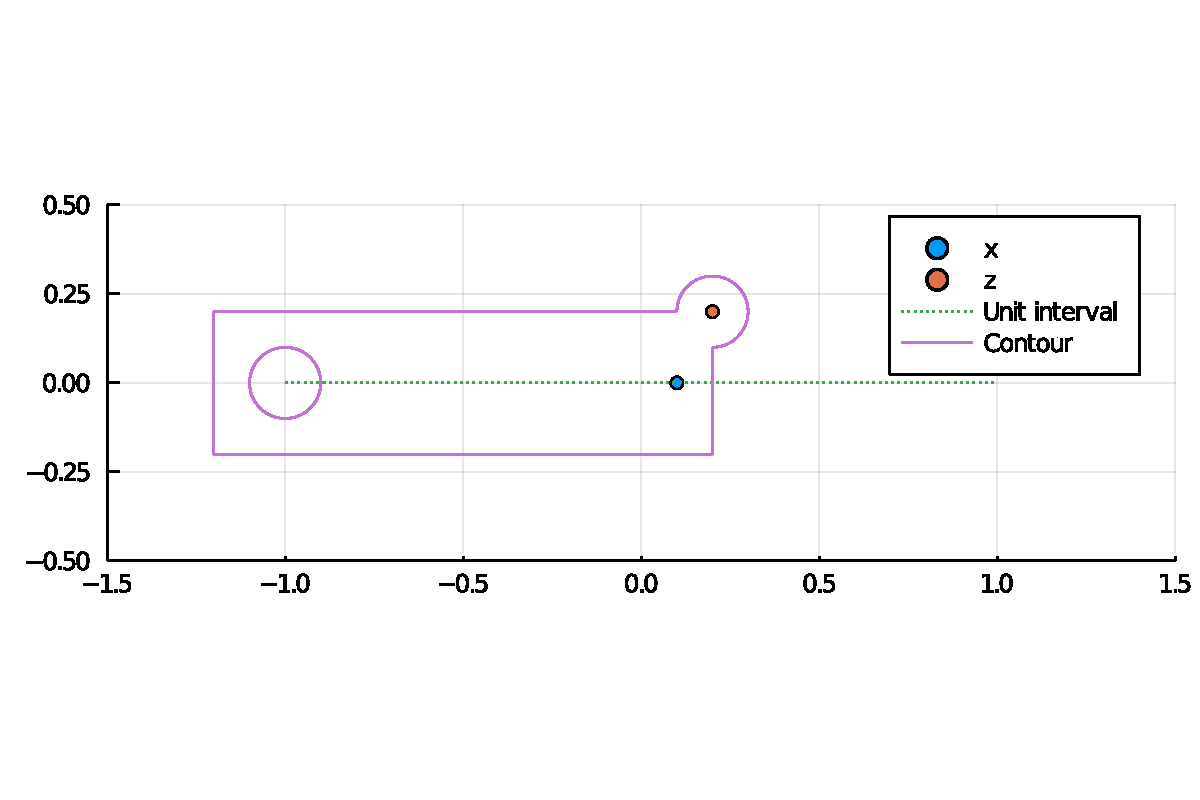
\includegraphics[width=0.8\linewidth]{C:/Users/mfaso/OneDrive/Documents/GitHub/M3M6AppliedComplexAnalysis/output/figures/Lecture10_11_1.pdf}}
This integral expression holds for all $z$ inside the contour $\tilde \Gamma_x$ but off the interval. But it therefore holds true for $f(x) = f_+(x) = f_-(x)$ by taking limits.  Thus $f(x) = {1 \over 2 \pi \I} \int_{{\tilde \Gamma}_x} {f(\zeta) \over \zeta -x} \D\zeta$ hence $f$ is analytic at $x$.\hfill \ensuremath{\mdblksquare}

In an upcoming lecture on the Cauchy transform, we'll encounter a function that has isolated singularities that are weaker than poles (according to the definitions in previous lectures, this is a contradiction in terms). We'll then need the following result which shows that we can analytically continue the function to such singularities via the Cauchy integral formula.

\textbf{Theorem (weaker than pole singularity implies analyticity)} Suppose $f$ is analytic in $D \backslash \{ z_0 \}$ and has a weaker than pole singularity at $z_0$:

\[
\lim_{z \rightarrow z_0} (z-z_0) f(z) = 0
\]
holds uniformly. Then $f$ is analytic at $z_0$. (More precisely: $f$ can be analytically continued to $z_0$.)
\newpage
\textbf{Proof}

Around $z_0$ is an annulus $A_{R0}$ inside which $f$ is analytic. Consider $z$ in $A_{R0}$ and a positively oriented circle $\gamma_r$ of radius $r$ with $|r| < |z-z_0|$. Then we have

\[
    f(z) = {1 \over 2 \pi \I} \oint_{\gamma_R} {f(\zeta) \over \zeta - z} \D \zeta - {1 \over 2 \pi \I} \oint_{\gamma_r} {f(\zeta) \over \zeta - z} \D \zeta .
\]
here's a plot:


\begin{lstlisting}
(*@\HLJLn{z\ensuremath{\_0}}@*) (*@\HLJLoB{=}@*) (*@\HLJLnfB{0.2}@*) (*@\HLJLoB{+}@*)(*@\HLJLnfB{0.2}@*)(*@\HLJLn{im}@*)
(*@\HLJLn{z}@*) (*@\HLJLoB{=}@*) (*@\HLJLnfB{0.4}@*) (*@\HLJLoB{+}@*)(*@\HLJLnfB{0.2}@*)(*@\HLJLn{im}@*)

(*@\HLJLnf{scatter}@*)(*@\HLJLp{([}@*)(*@\HLJLnf{real}@*)(*@\HLJLp{(}@*)(*@\HLJLn{z\ensuremath{\_0}}@*)(*@\HLJLp{)],[}@*)(*@\HLJLnf{imag}@*)(*@\HLJLp{(}@*)(*@\HLJLn{z\ensuremath{\_0}}@*)(*@\HLJLp{)];}@*) (*@\HLJLn{label}@*)(*@\HLJLoB{=}@*)(*@\HLJLs{"{}z{\_}0"{}}@*)(*@\HLJLp{)}@*)
(*@\HLJLnf{scatter!}@*)(*@\HLJLp{([}@*)(*@\HLJLnf{real}@*)(*@\HLJLp{(}@*)(*@\HLJLn{z}@*)(*@\HLJLp{)],[}@*)(*@\HLJLnf{imag}@*)(*@\HLJLp{(}@*)(*@\HLJLn{z}@*)(*@\HLJLp{)];}@*) (*@\HLJLn{label}@*)(*@\HLJLoB{=}@*)(*@\HLJLs{"{}z"{}}@*)(*@\HLJLp{)}@*)
(*@\HLJLnf{plot!}@*)(*@\HLJLp{(}@*)(*@\HLJLnf{Circle}@*)(*@\HLJLp{(}@*)(*@\HLJLn{z\ensuremath{\_0}}@*)(*@\HLJLp{,}@*) (*@\HLJLnfB{0.1}@*)(*@\HLJLp{);}@*) (*@\HLJLn{label}@*)(*@\HLJLoB{=}@*)(*@\HLJLs{"{}gamma{\_}r"{}}@*)(*@\HLJLp{,}@*)(*@\HLJLn{ratio}@*)(*@\HLJLoB{=}@*)(*@\HLJLnfB{1.0}@*)(*@\HLJLp{)}@*)
(*@\HLJLnf{plot!}@*)(*@\HLJLp{(}@*)(*@\HLJLnf{Circle}@*)(*@\HLJLp{(}@*)(*@\HLJLn{z\ensuremath{\_0}}@*)(*@\HLJLp{,}@*) (*@\HLJLnfB{0.3}@*)(*@\HLJLp{);}@*) (*@\HLJLn{label}@*)(*@\HLJLoB{=}@*)(*@\HLJLs{"{}gamma{\_}R"{}}@*)(*@\HLJLp{)}@*)
\end{lstlisting}

\cent{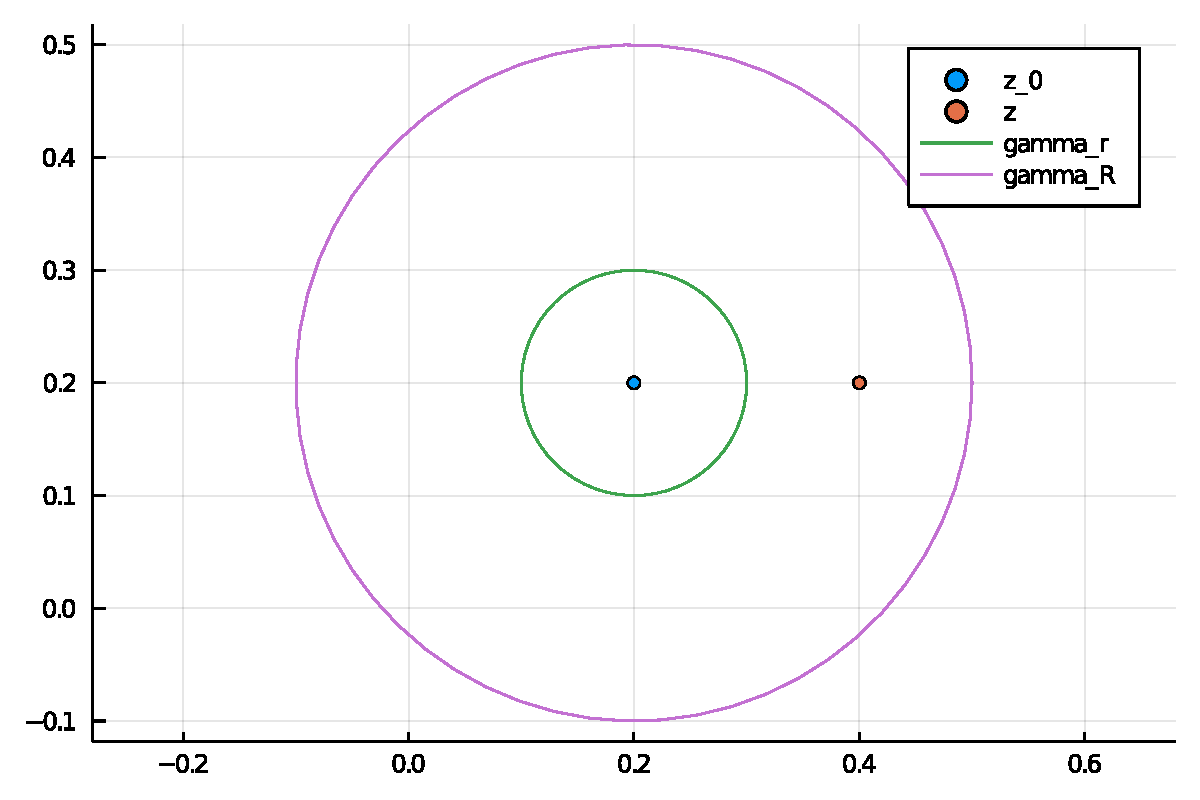
\includegraphics[width=0.8\linewidth]{C:/Users/mfaso/OneDrive/Documents/GitHub/M3M6AppliedComplexAnalysis/output/figures/Lecture10_12_1.pdf}}

But we have

\[
    \left|  \oint_{\gamma_r} {f(\zeta) \over \zeta - z} \D \zeta \right| \leq 2\pi r \sup_{\zeta \in \gamma_r} \left|{f(\zeta) \over \zeta - z}\right| \leq 2 \pi r  {1 \over |z_0-z| - r} \sup_{\zeta \in \gamma_r} |f(\zeta)|
\]
which tends to zero as $r \rightarrow 0$.

\ensuremath{\mdblksquare}

% 
% This can't be right because f = log(z) is a counterexample
% **Corollary (Weaker than linear growth implies analyticity at infinity)** If
% $$
% \lim_{z \rightarrow \infty} {f(z)  \over z} = 0,
% $$
% then $f$ is analytic at infinity.
% 
% 
% From these result we can infer that
% $$
% \phi(z) = \sqrt{z-1}\sqrt{z+1}
% $$
% is analytic on $\C \backslash [-1,1]$, and $\phi(z) \sim_{z \rightarrow \infty} z$.
%  

}
\end{document}
